\documentclass{article}
\usepackage{graphicx}
\usepackage[]{mdframed}
\usepackage{tabularx}
\usepackage{subfig}
\usepackage{placeins}
\usepackage{float}
\usepackage{amsmath}

\graphicspath{ {../images/} }
\usepackage[a4paper, total={6in, 8in}]{geometry}


\author{Sidharth Babu, SNB2593 \and Tianda Huang, TH32678}
\title{ECE 361E: Homework 2}

\begin{document}
\begin{mdframed}
    \maketitle
\end{mdframed}
\pagebreak

\section{Problem 1}

\subsection{Question 1}
\begin{figure} [!htb]
    \centering
    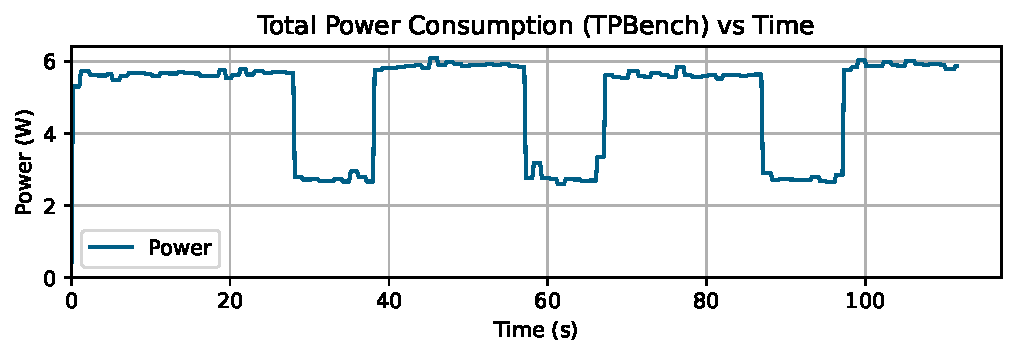
\includegraphics[scale=0.8]{tpb_power.pdf}
    \label{fig:tpb-power}
\end{figure}
\begin{figure} [!htb]
    \centering
    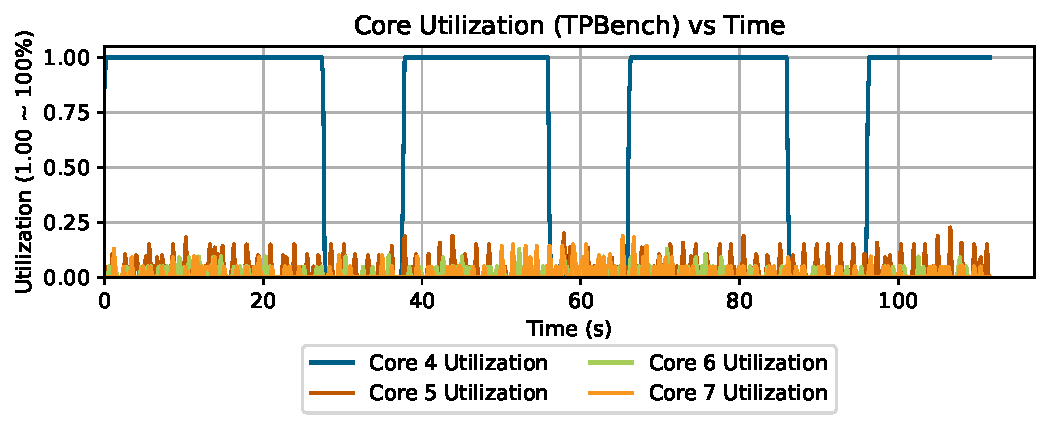
\includegraphics[scale=0.8]{tpb_util.pdf}
    \label{fig:tpb-util}
\end{figure}
\begin{figure} [!htb]
    \centering
    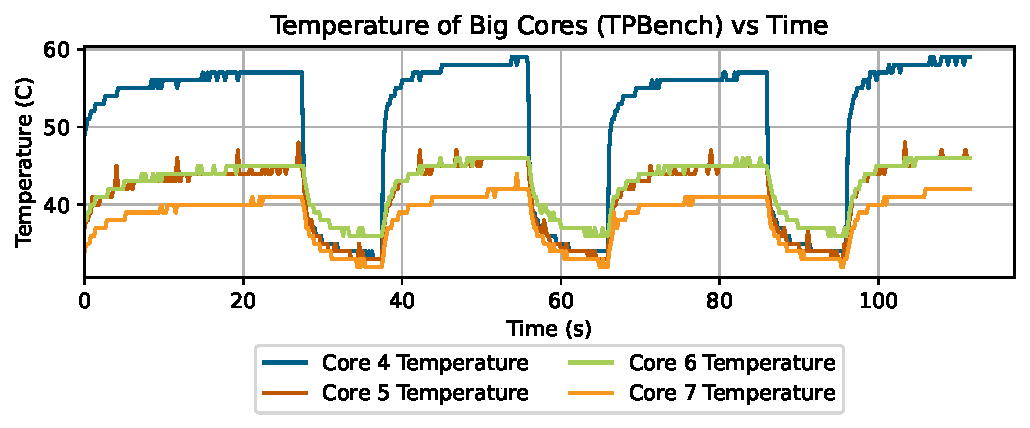
\includegraphics[scale=0.8]{tpb_temp.pdf}
    \label{fig:tpb-temp}
\end{figure}

\subsection{Question 2}
We can identify four major phases of the benchmark's execution, marked by sharp rises in temperature (and also power and utilization).

\subsection{Question 3}

\begin{figure} [!htb]
    \centering
    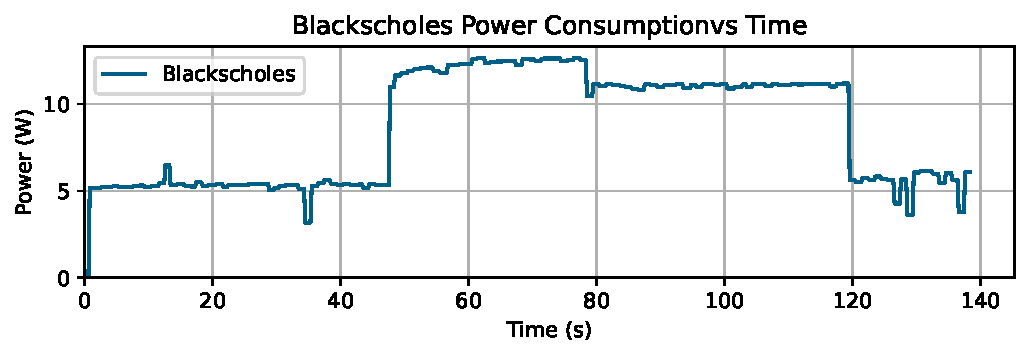
\includegraphics[scale=0.8]{blk_power.pdf}
    \label{fig:blk-power}
\end{figure}
\begin{figure} [!htb]
    \centering
    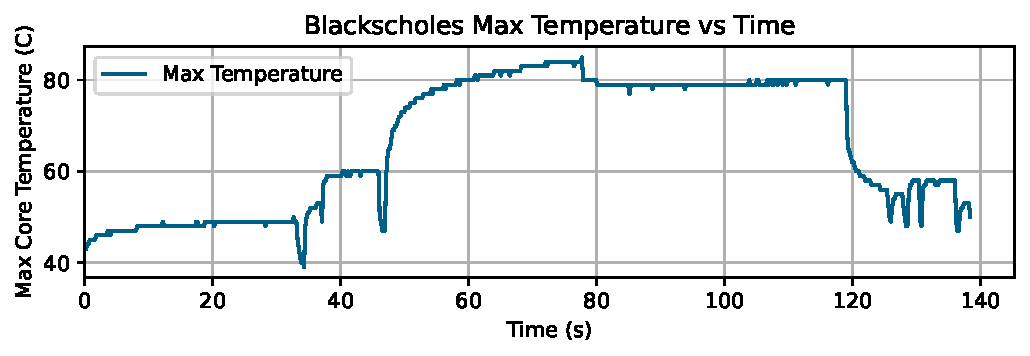
\includegraphics[scale=0.8]{blk_maxtemp.pdf}
    \label{fig:blk-maxtemp}
\end{figure}
\begin{figure} [!htb]
    \centering
    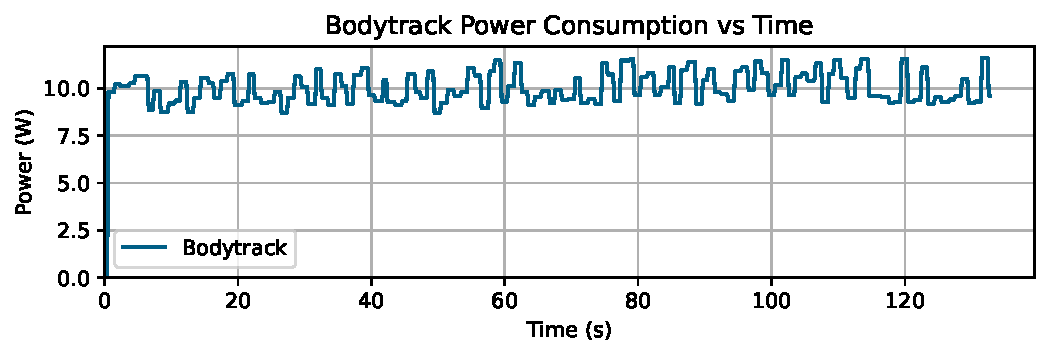
\includegraphics[scale=0.8]{body_power.pdf}
    \label{fig:body-power}
\end{figure}
\begin{figure} [!htb]
    \centering
    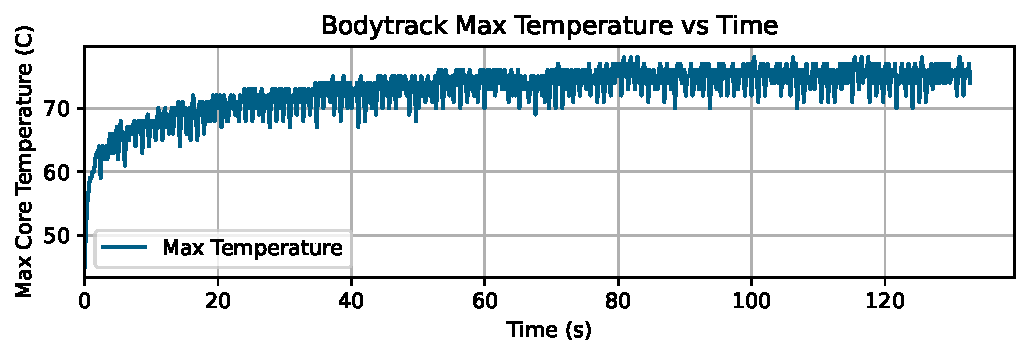
\includegraphics[scale=0.8]{body_maxtemp.pdf}
    \label{fig:body-maxtemp}
\end{figure}

\begin{figure} [!htb]
    \centering
    \caption{\textit{blackscholes} and \textit{bodytrack} Benchmark Results Table}
    \begin{tabular}[!htb]{|c|c|c|c|c|c|} \hline
        Benchmark & Run time [s] & Avg. power [W] & Avg. max temp [$^{\circ}$C] & Max temp [$^{\circ}$C] & Energy [J] \\ \hline
        \textit{\textbf{blackscholes}} & 138.41 & 8.55 & 66.21 & 85.00 & 42.60 \\ \hline
        \textit{\textbf{bodytrack}} & 132.78 & 9.97 & 72.77 & 78.0 & 49.62 \\ \hline
    \end{tabular}
    \label{fig:multithread-bench}
\end{figure}

\pagebreak

\section{Problem 2}

\subsection{Question 1}
Based on the near-perfect performance metrics and confusion matrix (i.e. only one missed prediction per testfile), the performance of the classifier could be considered 'excellent'. This is likely due to the 'total\_watts' parameter that represents a near-perfect metric of big-core wattage since we roughly have $$\text{total W} \approx \text{big-core W} + \text{little-core W} + \text{gpu W} + \text{memory W}$$

\begin{figure} [!htb]
    \centering
    \caption{\textit{blackscholes} and \textit{bodytrack} Confusion Matrix}
    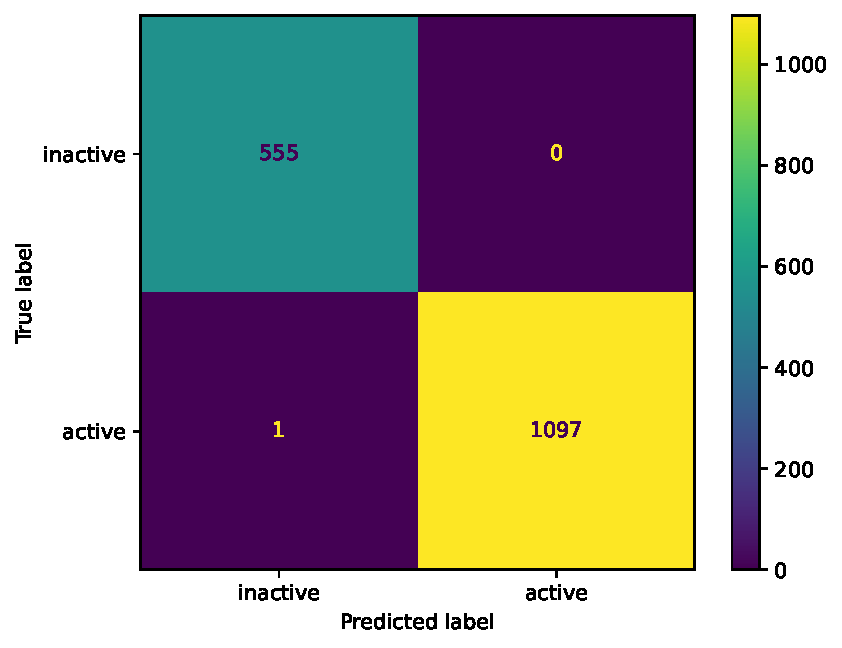
\includegraphics[scale=0.5]{blk_confusion.pdf}
    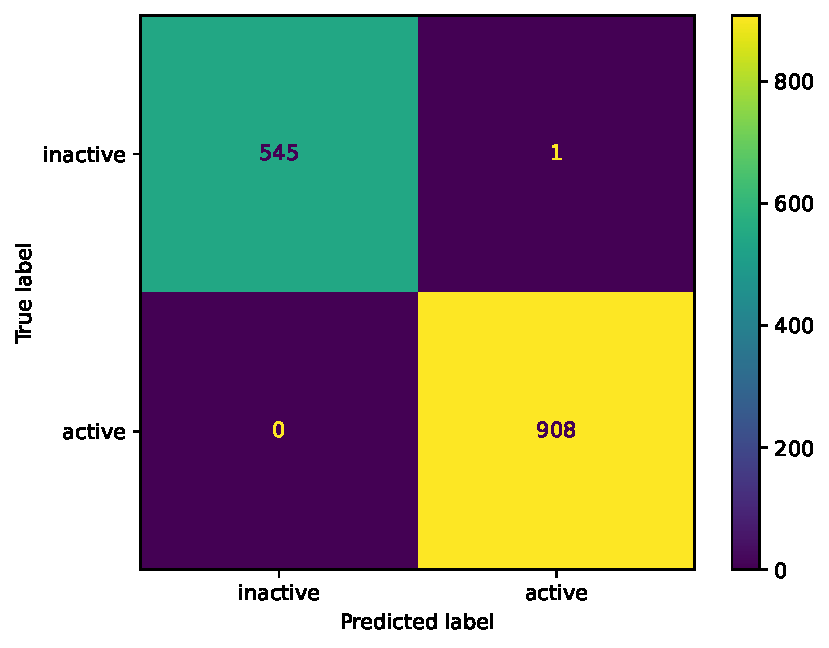
\includegraphics[scale=0.5]{body_confusion.pdf}
    \label{fig:blk-body-confusion}
\end{figure}

\begin{figure} [!htb]
    \centering
    \caption{\textit{blackscholes} and \textit{bodytrack} SVM Model Performance Metrics}
    \begin{tabular}[!htb]{|c|c|c|c|c|} \hline
        Benchmark & Accuracy & Precision & Recall & F1-Score \\ \hline
        \textit{\textbf{blackscholes}} & 0.999 & 1.000 & 0.999 & 1.000 \\ \hline
        \textit{\textbf{bodytrack}} & 0.999 & 0.999 & 1.000 & 0.999 \\ \hline
    \end{tabular}
    \label{fig:power-svm}
\end{figure}

\pagebreak

\subsection{Question 2}

\begin{figure} [!htb]
    \centering
    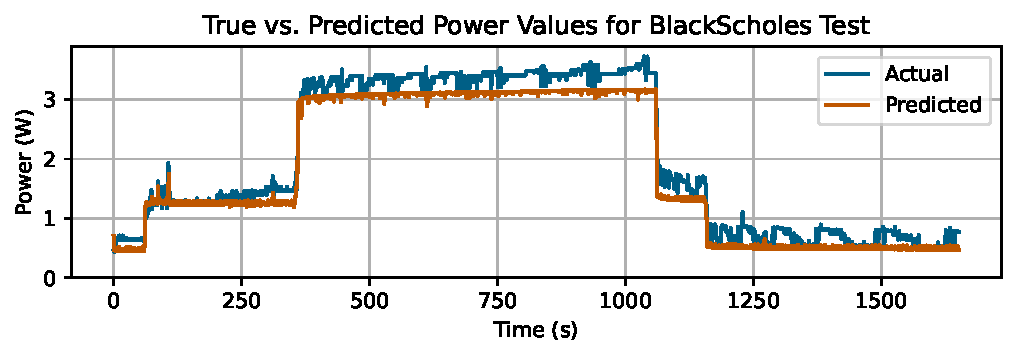
\includegraphics[scale=0.8]{blackscholes_linreg.pdf}
    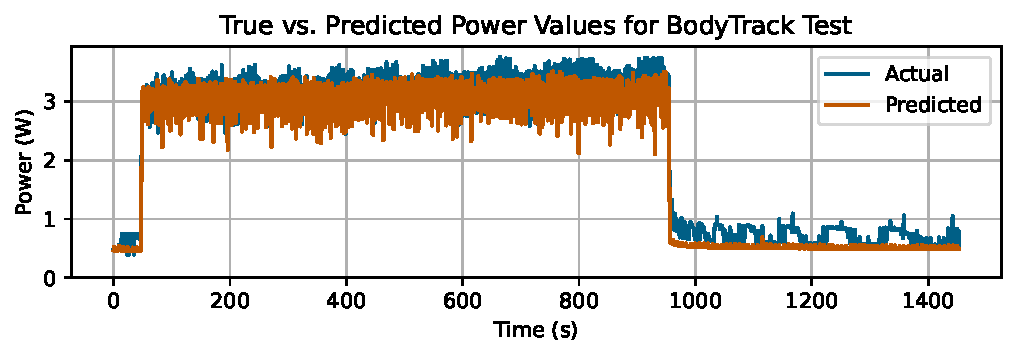
\includegraphics[scale=0.8]{bodytrack_linreg.pdf}
    \label{fig:blk-body-linreg}
\end{figure}

\begin{figure} [!htb]
    \centering
    \caption{Wattage Linear Regression Model Performance}
    \begin{tabular}[!htb]{|c|c|c|c|} \hline
        Dataset & \textit{\textbf{training}} & \textit{\textbf{blackscholes}} & \textit{\textbf{bodytrack}} \\ \hline
        $\text{R}^2$ & 0.987 & 0.957 & 0.922 \\ \hline
        MSE & 0.010 & 0.059 & 0.122 \\ \hline
    \end{tabular}
    \label{fig:power-linreg}
\end{figure}

\subsection{Question 3}
Dynamic power, big cluster frequency, and GPU temperature are the features with the highest magnitude (and thus the largest contribution to the linear regressor). We can see that in general, frequency and its derived parameter dynamic power are the best features, followed by temperature, then followed by usage. This is likely due to dynamic power being a major component in total power draw. Temperature is an effect of increased power draw and thus lags behind when observing the data; this means that temperature is a relatively good feature.

\begin{figure} [!htb]
    \centering
    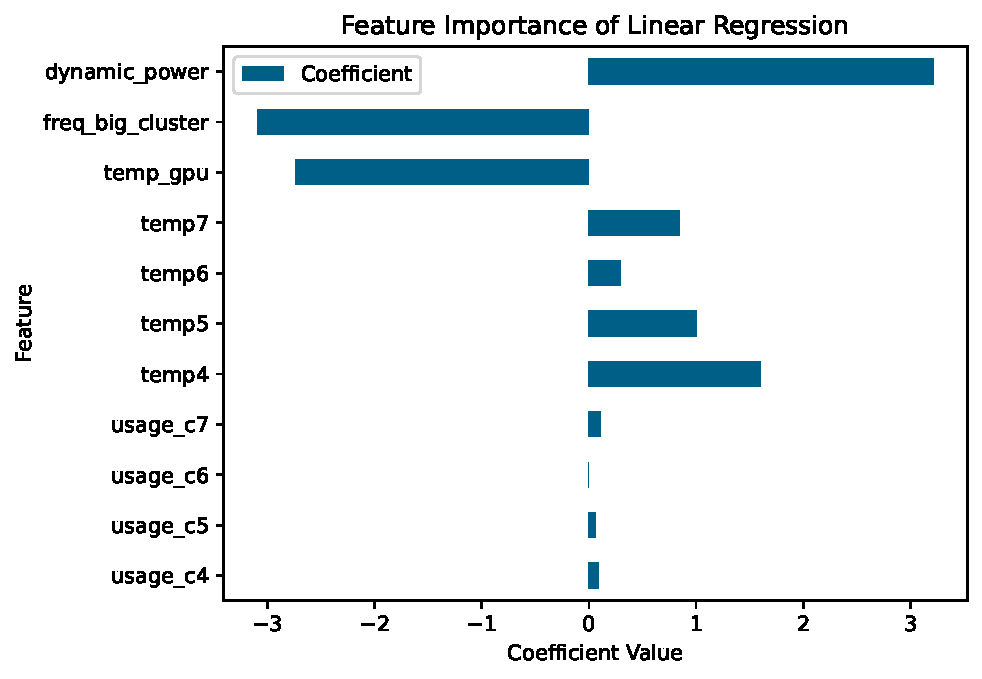
\includegraphics[scale=0.8]{linreg_importance.pdf}
    \label{fig:linreg-importance}
\end{figure}

\section{Problem 3}

\subsection{Question 1}

\begin{figure} [!htb]
    \centering
    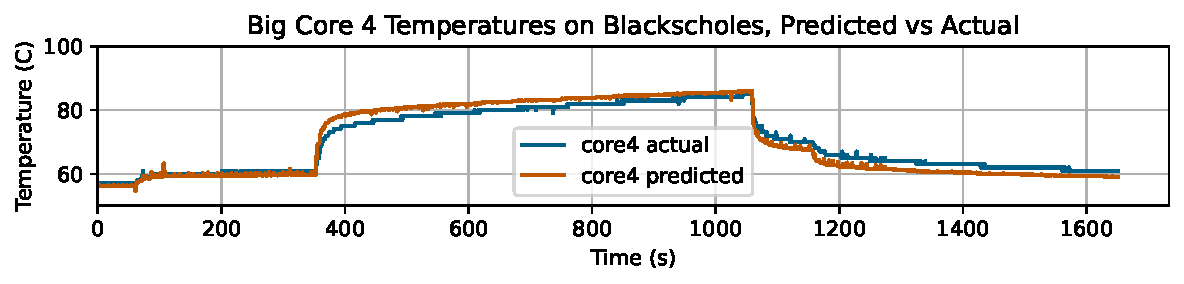
\includegraphics[scale=0.8]{blk_mlp.pdf}
    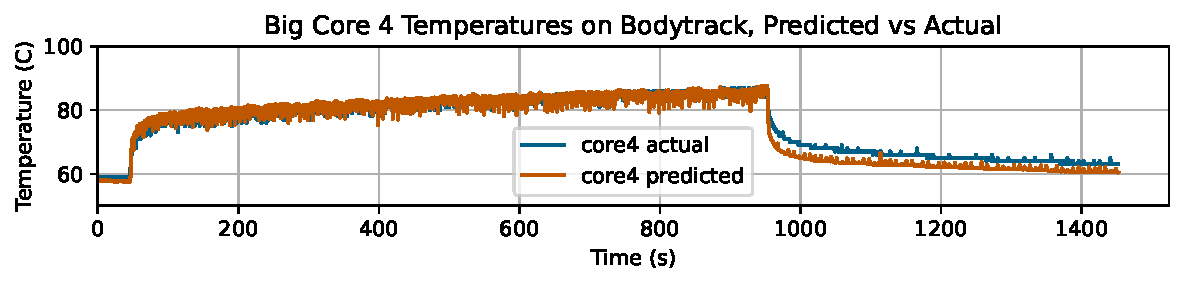
\includegraphics[scale=0.8]{body_mlp.pdf}
    \label{fig:blk-body-mlp}
\end{figure}

\begin{figure} [!htb]
    \centering
    \caption{Temperature MLPRegressor MSE ($\text{C}^2$)}
    \begin{tabular}[!htb]{|c|c|c|c|c|} \hline
        Dataset & Test MSE (Core 4) & Test MSE (Core 5) & Test MSE (Core 6) & Test MSE (Core 7) \\ \hline
        \textit{\textbf{blackscholes}} & 5.18 & 6.11 & 6.22 & 3.78 \\ \hline
        \textit{\textbf{bodytrack}} & 5.76 & 7.24 & 7.42 & 6.84 \\ \hline
    \end{tabular}
    \label{fig:temp-mlp}
\end{figure}

\subsection{Question 2}
The first major technique for improving performance is by including more past temperature data when estimating the next temperature step. As the processor elements contain some thermal mass, temperature will continue to rise even as power drops, and fast spikes in usage and power may not be reflected in a temperature increase in the very next time step. Thus, by including more past temperatures in calculating the next, we can account for this delay in temperature response.\\

Second, from a model perspective, increasing the number of nodes in the MLP can marginally increase the performance.

\subsection{BONUS Question 3}
An on-demand governor such as the PI-controller listed can save more energy at the cost of an increase in runtime. A higher temperature decreases efficiency in the MCU due to higher static power and increased resistances, resulting in worse performance-per-watt metrics. However, a lower temperature ceiling results in lower total performance, which increases runtime.\\

The tradeoff between better performance/runtime and better performance-per-watt cannot be simply solved by reducing temperature as much as possible: past a certain point, the increased time from a lower temperature/power draw results in higher total energy compared to the inefficient power/high performance case.

\section{Contributions and Valuable Things Learned}
Both group members, Sidharth Babu and Tianda Huang, contributed an equal amount of work due to working on the entire project together.\\

We learned about the power and temperature implications of running high workloads on an single-package SOC, including the temperature-bleed effects of running cores/functional units on physically adjacent cores/functional units.\\

On the data science and machine learning side, we learned about the importance of scaling input features (linearly and non-linearly) regarding achieving maximum performance from a model.

\end{document}